\section{Background}
\label{sec:background}

%% In this section, we briefly review the browser architecture and
%% security model.
%
\iffigures
\begin{figure}
%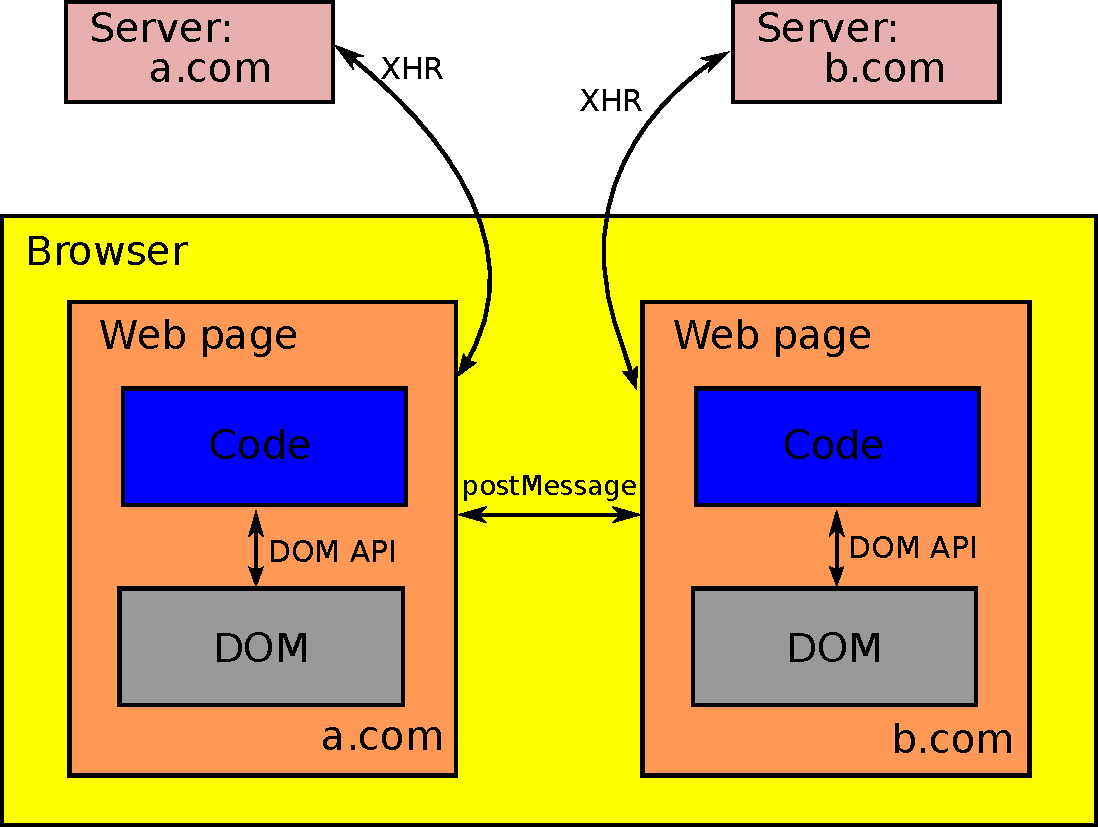
\includegraphics[width=\columnwidth]{setting.pdf}
\begin{center}
% I printed out, and it reads well!
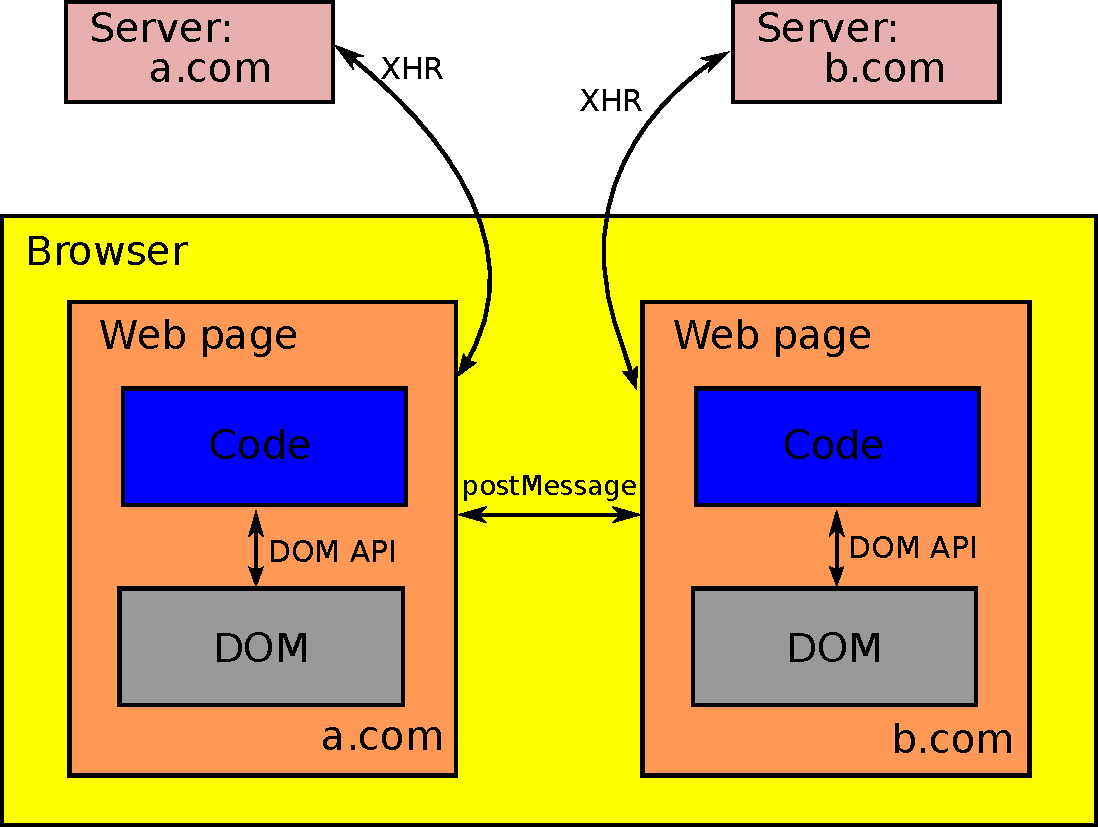
\includegraphics[scale=0.35]{setting.pdf}
\end{center}
\vspace{-10pt}
\caption{\label{fig:browser-arch} Browser architecture model}
\vspace{-10pt}
\end{figure}
As shown in Figure~\ref{fig:browser-arch}, a 
\else
A
\fi
web page is composed of
content and JavaScript code.
%
The browser provides an environment, called the \emph{browsing
context}, within which the page's content is presented to the user and
made accessible to JavaScript code through the \emph{Document Object
Model (DOM)}~\cite{html5}.
%
Within this context, the content/code may create and interact with
nested browsing contexts (e.g., iframes), use persistent storage
(e.g., cookies) or perform network requests (either implicitly through
content loading or explicitly, in JavaScript, using the \xhr{} (XHR)
constructor).
%
Since different components may be provided by different authors, it is
important that these complex interactions abide by a security policy.
 
Policies are expressed in terms of \emph{origins}; an origin is a
source of authority encoded by the protocol (e.g., \js|http|), domain
name (e.g., \js|fb.com|), and port (e.g., \js|443|) of a resource
URL.\footnote{
  While at least the protocol is necessary to describe an
  origin, for brevity, we assume that the protocol and port are
  respectively \js|https| and \js|443| and omit them from URLs.
}
%
Below we briefly review the core browser security policies, including
the Same-Origin Policy~\cite{rfc6454}, Content Security
Policy~\cite{csp}, and Cross-Origin Resource Origin
policy~\cite{cors13}.
%
%
We note that our review is not exhaustive (e.g., among other, we not
discuss the \js|X-Frame-Options| header, which prevents loading a page
in a nested browsing context);  the interested reader is referred
to~\cite{googlehandbook} for a more complete discussion on web security.



\subsection{Same-Origin Policy}
\label{sec:background:sop}

The SOP specifies that resources of an origin should only be readable
by content from the same origin~\cite{rfc6454, googlehandbook,
VanKesteren2012}.
%
Hence, browsers ensure that code executing in a \https{a.com} context
can only inspect the DOM and cookies of another context if they share
the same \https{a.com} origin.
%
Similarly, the code can only inspect the response of a network
request---performed with XHR---if the remote host's origin is
\https{a.com}.
%
%% In general, the SOP isolates code in one page from accessing client-
%% and server-side data associated with another origin.
 
The SOP does not, however, prevent code from disclosing data to
foreign origins.
%
For example, code executing in an \https{a.com} context can trivially
disclose data to \https{b.com} by using XHR to perform a network
request; the SOP only prevents the code from inspecting the response
of such XHR requests, it does not impose any restrictions when sending
the request.
%
Similarly, code can exfiltrate data by encoding it in the path of a
URL, whose origin is \https{b.com}, and setting the \js|src| property
of an \js|img| element to this URL.

More generally, the ability to embed content from an arbitrary origin
can also be used to communicate data back into the page and ``bypass''
SOP's goal of disallowing cross-origin reads.
%
This is possible because most content is not completely opaque. 
%
For example, images can encode data in properties such as width and
height (which are always readable), scripts can encode data in their
execution sequence (as done by JSON-P~\cite{jsonp}), etc.
%

The popularization of JSON-P and other ad-hoc cross-origin
communication methods, (notably, those relying on \js|window.name| and
\js|window.location|~\cite{thidpartyjs}), has lead to the introduction
of the HTML5 \js|postMessage| API~\cite{webmessaging}.
%
This API allows code from different browsing contexts to exchange
messages, as shown in Figure~\ref{fig:browser-arch}.
%
Given a foreign-origin DOM window object \js|win|, the
\js|postMessage| method can be invoked on it to send the
foreign-origin a message: \js|win.postMessage(message, destOrigin)|.
%
Since browsing contexts can be navigated, to prevent man-in-the-middle
attacks~\cite{barth2009securing}, a second argument
\js|destOrigin| is used to specify the intended origin of the message.
%
Unfortunately, once the message is sent to the foreign-origin browsing
context, the page has no control over what the origin can do with the
data.
%
Hence, sending sensitive data using \js|postMessage| should only be
done if the foreign-origin is trusted;
%
in Section~\ref{sec:system:iframe}, we describe how \sys{} precisely
allows code to impose restrictions on where the foreign-origin can
disseminate data received via \js|postMessage|, removing this need for
complete trust.

\subsection{Content Security Policy} 
\label{sec:background:csp}

Addressing cross-site scripting (XSS) attacks~\cite{kerschbaum2007simple}, CSP
provides developers with a means for white-listing the origins from which their
application is allowed to load resources~\cite{csp}.
%
Specifically, when first loading a page, the
\js|Content-Security-Policy| header is inspected for directives that
instruct the browser to limit the browsing context to loading
specific resources from the provided white-lists.
%
For instance, if the CSP header of a page from \https{a.com} contains
the following three directives
%
\texttt{default-src 'self'}, \texttt{img-src 'none'}, and
\texttt{connect-src https://b.com},
%
the page content loading is restricted as follows.
%
First, loading resources---for which a more specific directive is not
provided (e.g., scripts, stylesheets, etc.)---is limited to the same
origin (\texttt{'self'}).
%
Second, the context is prohibited from loading any images
(\texttt{'none'}).
%
And, third, JavaScript code is restricted to making XHR requests to
\https{b.com}.

Although the CSP specification only states that attempts to load
resources from origins outside the white-list should behave as if the
remote server responded with a failure (HTTP 400) response, most
browsers do not actually perform requests.
%
Hence, in addition to addressing XSS attacks, in practice, CSP can be
used to partially restrict the origins to whom data can be exfiltrated
by malicious code executing in the browsing context---recall that all
code within a page has the authority of the page, regardless of the
source origin.
%
Unfortunately, CSP only gives developers the choices of trusting code
to communicate with an origin in full or not at all;
%
in Section~\ref{sec:system:worker} we show how \sys{} overcomes this
shortcoming to allow code to communicate with an arbitrary untrusted
origin until it reads sensitive data.


\subsection{Cross-Origin Resource Sharing} 
\label{sec:background:cors}

While CSP tightens down the SOP by restricting reads and writes, CORS
loosens the restrictions imposed by the SOP~\cite{rfc6454, VanKesteren2012,
googlehandbook}.
%
Specifically, CORS allows web servers to specify, using a header that
white-lists origins, which browsing contexts are allowed to inspect
the content of a resource.
%
Suppose, for instance, that code executing in an \https{a.com} browsing
context makes an XHR request to \https{b.com}.
%
Normally, the SOP would prevent the code from inspecting the response.
%
However, if the response contains the CORS header
\texttt{Access-Control-Allow-Origin: https://a.com}, the browser will
not restrict the JavaScript code from reading the actual response
content.

CORS addresses the limitations of SOP in allowing cross-origin
sharing and overcomes the need for ad-hoc sharing methods such as
JSON-P.
%
However, CORS, like CSP, requires resource providers to, a-prior,
declare an all-or-nothing trust relationship.
%
Though this is sufficient for certain scenarios (e.g., making a
resource public, or sharing content between origins owned by a single
entity) in many cases it is overly restricting and rigid;
%
in Section~\ref{sec:system:mashup} we show how \sys{} overcomes this
shortcoming by allowing code to read arbitrary cross-origin
data in a safe and controlled manner.


% Local Variables:
% TeX-master: "main.ltx"
% TeX-command-default: "Make"
% End:

